\documentclass{article}

\usepackage{coursenotes}

\set{AuthorName}{TC Fraser}
\set{Email}{tcfraser@tcfraser.com}
\set{Website}{www.tcfraser.com}
\set{ClassName}{Topics in Condensed Matter}
\set{School}{University of Waterloo}
\set{CourseCode}{Phys 435}
\set{InstructorName}{Anton Burkov}
\set{Term}{Winter 2017}
\set{Version}{1.0}

\draftprofile[TC Fraser]{TC}{Red}

\begin{document}

\titlePage

\tableOfContents

\disclaimer

\section{Toy Model of a Solid}

\todo[TC]{Type up notes for first class}

Thus far we have been discussing a toy model of a solid in one dimension. By diagonalizing the Hamiltonian we were able to determine the energy levels of the various states,
\[ \varepsilon\br{k} = - 2 t \cos\br{ka} \]
Where $k$ is the wave-vector with $p = \hbar k$ as the ordinary linear momentum. Additionally, $t$ acts as a tunneling coefficient that dictates a tunneling \textit{rate} (up to a constant $\hbar$) for the electrons in the solid. Unlike free particles, the momentum $k$ in this toy model is confined to a discrete region.
\[ -\f{\pi}{a} \leq k < \f{\pi}{a} \]
This interval is called the \term{first Brillouin zone}.
To highlight this difference, we sometimes refer to $p$ in this model as the \term{crystal momentum}.\\

Moreover, the periodic boundary conditions used restrict $k$ to take on discrete and finite values,
\[ k = \f{2 \pi m}{N} \qquad m = 0, \pm 1, \pm 2, \ldots \]
Where $L = Na$ is the size of the crystal, $N$ is the number of atoms and $a$ is the interval between two atoms in the solid.\\

The states that diagonalized the Hamiltonian are called \term{Bloch states} and are denoted $\ket{k}$ where,
\[ \ket{k} = \f{1}{\sqrt{N}} \sum_{n} \ket{n} e^{i k na} \]
Which is a \term{lattice Fourier transform}. Since $k$ is confined to a finite interval, the energy levels are confined to a finite interval,
\[ \varepsilon_{\min} = - 2t \qquad \varepsilon_{\max} = + 2t \]
The interval has a width of $\varepsilon_{\max} - \varepsilon_{\min} = 4t$ and is referred to as the allowed energy \textit{band}.

\begin{center}
\begin{tikzpicture}
    \pgfmathsetmacro{\axissize}{4};
    \pgfmathsetmacro{\plotsize}{3};
    \draw[->] (-\axissize,0) -- (+\axissize,0) node[right]{$k$};
    \draw[->] (0, -\axissize) -- (0,+\axissize) node[above]{$\vep\br{k}$};
    \draw[scale=1.0,domain=-pi:pi,smooth,variable=\k,red] plot ({\k/pi*\plotsize},{-2*cos(deg(\k))});
    \draw[dashed] (\plotsize, -\axissize) -- node[above right]{$\f{\pi}{a}$} (\plotsize,+\axissize);
    \draw[dashed] (-\plotsize, -\axissize) -- node[above left]{$-\f{\pi}{a}$} (-\plotsize,+\axissize);
    \draw[-] (-0.1,-2) -- (+0.1,-2) node[right]{$-2t$};
\end{tikzpicture}
\end{center}

How many states does the band contain. Given that $k$ is discrete and bounded,
\[ -\f{\pi}{a} \leq \f{2 \pi m}{Na} = k < \f{\pi}{a} \]
Implies,
\[ -\f{N}{2} \leq m < \f{N}{2} \]
Therefore there are $N$ distinct waves of $m$. The total number states per band is thus $2N$ where $N$ is the number of primitive unit cells in the crystal.\\

Suppose now that we have $1$ electron per atom (instead of $1$ electron in total). We recall the \term{Pauli principle} which states that only $1$ electron can occupy a given state in a band. Since there are $N$ electrons and $2N$ states, the band is \textit{half-filled}.
\begin{center}
\begin{tikzpicture}
    \pgfmathsetmacro{\axissize}{4};
    \pgfmathsetmacro{\plotsize}{3};
    \draw[->] (0,0) -- (+\axissize,0) node[right]{$T$};
    \draw[->] (0, 0) -- (0,+\axissize) node[above]{$\rho\br{T}$};
    \draw[scale=1.0,domain=0.25:\plotsize,smooth,variable=\T,red] plot ({\T},{1/\T});
\end{tikzpicture}
\end{center}

When the electrons occupy all of the lowest possible energy states, we fill all of the negative energy states and the positive energy states remain vacant. This separation defines the \term{Fermi energy} for this system where occurs at $\vep\tsb{F} = 0$. In order to find the state that corresponds to this upper limit one needs to solve,
\[ \vep\br{k} = \vep\tsb{F} = 0 \implies -2t \cos\br{ka} = 0 \]
Therefore the value of $k$ that solves this equation is,
\[  k = \pm \f{\pi}{2a} = \pm k\tsb{F}\]
Where $k\tsb{F}$ is given a special name: the \term{Fermi wave-vector} (Fermi momentum).
\begin{align*}
    \abs{k} < k\tsb{F} &: \text{filled states}\\
    \abs{k} > k\tsb{F} &: \text{empty states}
\end{align*}
The \term{Fermi surface} defines the surface in momentum space separating the filled states from the unfilled states. Most of the observed properties of metals follow from the existence of the Fermi surface. \\

This concept is so important that it is worth measuring the volume \text{in momentum space} corresponding to the filled states. This is the volume enclosed by the Fermi surface. In this example, the volume in momentum space is characterized by the $2 k\tsb{F}$ interval. Since $k = 2\pi m / Na$, the volume per single $k$-value is $2 \pi / Na$. Letting $n$ be the density of electrons, we can compute the total number of electrons:
\[ n N a = 2 \f{2k\tsb{F}}{2 \pi / Na} \]
Which allows one to calculate $k\tsb{F}$,
\[ k\tsb{F} =\f{\pi}{2} n \]
Which makes sense for this model because there is one electron per atom making $n = 1/a$.
This result is called \term{Luttinger's theorem} which states that the volume enclosed by the Fermi surface (sometimes called the Fermi sea) is directly proportional to the electron density. \\

This toy model actually describes a real solid called polyacetylene. Polyacetylene consists of weakly-interacting chains of CH units.
\begin{align*}
    \text{C} &: 1s^2 2s^2 2p^2 \qquad \text{4 valence electrons}\\
    \text{H} &: 1s^1
\end{align*}

Electrons found in the inner orbitals of the atoms are tightly bound to their nuclei and therefore only the valence electrons in carbon are free to travel throughout the lattice.

\begin{center}
    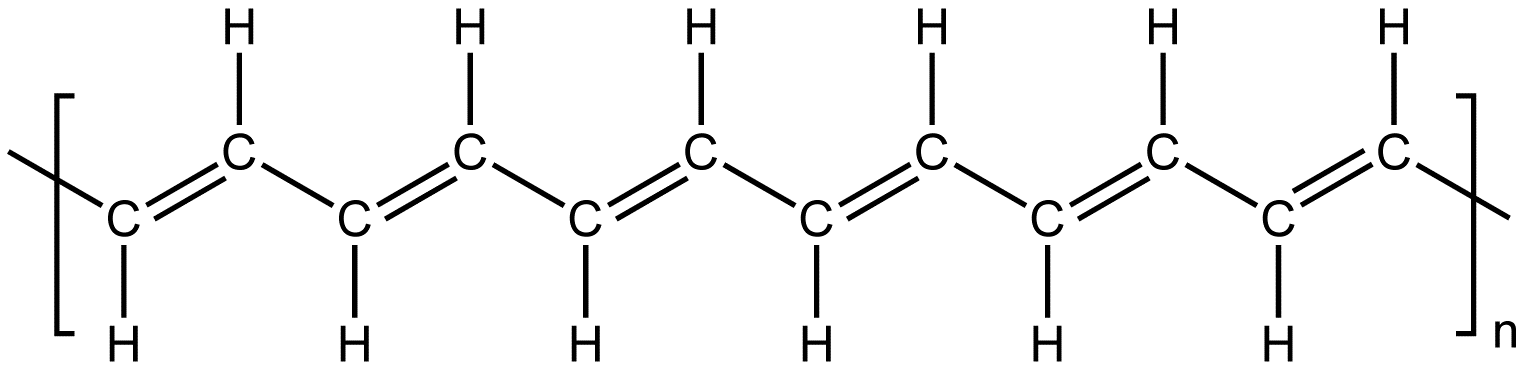
\includegraphics[width=\linewidth]{figures/polyacetylene.png}
\end{center}

Three of the valence electrons are engaged in bonding with neighboring carbon and hydrogen atoms while the $4$-th one is free to move around. As it turns out, the bonds between carbon atoms possess alternating tunneling amplitudes.

\begin{center}
    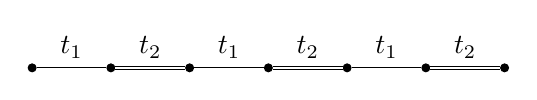
\begin{tikzpicture}
        \foreach \i in {1,...,7}
        {
            \node[draw, fill, circle, inner sep=1pt] (\i) at (\i,0) {};
        }
        \draw[]       (1) -- node[above]{$t_1$} (2);
        \draw[double] (2) -- node[above]{$t_2$} (3);
        \draw[]       (3) -- node[above]{$t_1$} (4);
        \draw[double] (4) -- node[above]{$t_2$} (5);
        \draw[]       (5) -- node[above]{$t_1$} (6);
        \draw[double] (6) -- node[above]{$t_2$} (7);
    \end{tikzpicture}
\end{center}


\end{document}
